\documentclass[xcolor=table,10pt,t]{beamer}
\title{CLAM}
\subtitle{From NLP command-line tools to webservices: current state of affairs}
\date{\today}
\author{Maarten van Gompel}
%% Use the official themes as much as possible
%\usetheme[official=false,department=clst]{ruhuisstijl}
%\usetheme[official=false]{ruhuisstijl}
\usetheme[official=true,department=clst]{ruhuisstijl}


\begin{document}

\begin{frame}
    \titlepage{}
        \begin{figure}
        \includegraphics[height=1cm]{clamup_bw.png}
        \end{figure}
        \vspace{3.5cm}
    \includegraphics[width=5cm]{lama-logo-transparent.png}
\end{frame}



\begin{frame}{Introduction}
  \begin{block}{}
    \textbf{Observation:} NLP tools are often command-line programs \ldots for
    good reason.
  \end{block}
\end{frame}



\begin{frame}{Command line tools: pros}
  \begin{block}{Command-line tools are a good thing!}
      \emph{``This is the Unix philosophy: Write programs that do one thing and do
      it well. Write programs to work together.'' (Doug McIlroy)}

      \medskip

      \begin{itemize}
        \item \textbf{Flexibility \& Extensibility}: Integrate tools into pipelines, the output of one tool is the input to another
        \item \textbf{Performance \& Simplicity}: Little overhead
        \item \textbf{Modularity}: Separate the interface (GUI, web) from the actual program
      \end{itemize}

  \end{block}

\end{frame}


\begin{frame}{Command line tools: cons}
  \begin{block}{But\ldots}
      \begin{itemize}
        \item The command-line is challenging and intimidating for non-technical end-users
        \begin{figure}
            \includegraphics[height=4cm]{commandlinefear.jpg}
        \end{figure}
        \item \textbf{Installation}: Installation may complex and depend on other software
        \item \textbf{Connectivity}: Web-connectivity/networking has to be
            explicitly built-in into your program (not trivial)
      \end{itemize}
  \end{block}
\end{frame}

\begin{frame}{Web-connectivity through CLAM}
  \begin{block}{Objectives}
      \begin{itemize}
        \item Quickly transform existing command-line tools into fully-fledged webservices
        \begin{itemize}
            \item No need to alter the tool itself
            \begin{itemize}
                \item \footnotesize{No requirements on programming language or technology, as
                long as it runs on Linux/BSD and can be invoked from the command line}
            \end{itemize}
            \item Maintain flexibility and modularity
            \item Simply describe the tool in terms of input, output and
                parameters using CLAM
        \end{itemize}
        \item Offer a generic \textbf{RESTFUL interface} for machines
        \item Offer a generic \textbf{Web-based User Interface} for human end-users
        \item Deal with batch processing and large data: NLP tasks may typically run for a
            long time on large corpora
      \end{itemize}
  \end{block}
\end{frame}


\begin{frame}{Architecture}

    \begin{center}
    \includegraphics[width=70.0mm]{clamup.png}
    \end{center}

\end{frame}


\begin{frame}{Architecture}

    \begin{center}
    \includegraphics[width=70.0mm]{architecture2015_1.png}
    \end{center}

\end{frame}

\begin{frame}{Architecture}

    \begin{center}
    \includegraphics[width=70.0mm]{architecture2015_0.png}
    \end{center}

\end{frame}


\section{Providing a Service}

\subsection{Providing a Service}

\begin{frame}
    \begin{block}{Providing a Service (1/2)}
        In order to wrap a tool and make a webservice: \\
        \textbf{1.} Write a service configuration file
        \begin{itemize}
            \item General meta information about your system
                {\footnotesize{(name, description, etc\ldots)}}
            \item Definition of global parameters accepted by your system
            \item The program to invoke {\footnotesize{(i.e.\ the wrapper script around your NLP tool)}}
            \item Definition of \emph{profiles}
            \begin{itemize}
                \item A profile defines in detail what output files a system
                    produces given certain input files.
            \end{itemize}
        \end{itemize}

    \end{block}

\end{frame}

\begin{frame}
    \begin{block}{Providing a Service (2/2)}
        In order to wrap a tool and make a webservice: \\
        \textbf{2.} Write a wrapper script for your system
        \begin{itemize}
            \item Wrapper script is invoked by CLAM, and should in turn invoke the actual system
            \item Acts as glue between CLAM and your NLP Application.
            \item Can be written in any language (python users may benefit from the CLAM API)
            \item Not always necessary, simpler command-line applications can be invoked directly by CLAM as well.
        \end{itemize}
    \end{block}

    \begin{block}{Development}
        CLAM has a built-in webserver so it can be tested quickly in
        development.
    \end{block}

\end{frame}

\begin{frame}
    \begin{block}{Profiles}
        \begin{itemize}
            \item \textbf{What output files are produced given which input files?}
            \item What format are the input files in? (CLAM needs not be able to parse it itself)
            \item What parameters (metadata) are required or possible on input files?
            \item How is metadata propagated from input files to output files?
            \item What viewers are associated with output files?
            \item Which converters can act upon input/output files?
        \end{itemize}
    \end{block}
    \includegraphics[width=40.0mm]{blokkendoos.jpg}
\end{frame}



\begin{frame}{Resources}
  \begin{block}{Resources}
      \begin{itemize}
          \item \textbf{Projects}: Stored on server, owned by a user, each corresponds to a single
              run of the tool
          \begin{itemize}
            \item \textbf{Global parameters}: Parameters for the run
            \item \textbf{Input files}: Upload files or choose from preset collections on the server
            \begin{itemize}
                \item Local parameters (i.e.\ metadata)
            \end{itemize}
            \item \textbf{Output files}: Can be downloaded as-is, visualised
                using a \emph{viewer} or external webservice.
          \end{itemize}
      \end{itemize}
  \end{block}
\end{frame}


\begin{frame}{Workflow}
  \begin{block}{Typical Workflow}
      \begin{enumerate}
        \item Authentication
        \item Create a new project
        \item Upload files (and set per-file parameters if applicable)
        \item Set global parameters
        \item Start the project
        \item Wait for completion
        \item Download/view output files
        \item Delete project
      \end{enumerate}
  \end{block}
\end{frame}


\begin{tussenpagina}{}{}{screenshot_wide.png}
\end{tussenpagina}

\begin{frame}{Projects vs Actions}
    \begin{block}{Projects: Batch processing}
      \begin{itemize}
        \item CLAM is optimised for \textbf{batch processing}, your tool may run for hours or days if necessary
        \item The user can always close his browser and come back later
        \item Data stored and held on server until explicitly deleted
        \item Different from real-time request-response cycles
      \end{itemize}
    \end{block}

    \begin{block}{Actions: Real-time response}
      \begin{itemize}
        \item Define a command line application or Python function to run for a specific webservice URL
        \item Independent of projects
        \item Extensive parameter specification (but no file upload!)
        \item Command/function is expected to return a result in a short time interval
        \item Output of command/function is returned by CLAM to the user/client
      \end{itemize}
    \end{block}
\end{frame}


\begin{frame}{Authentication}
  \begin{block}{Authentication}
      \begin{itemize}
        \item Projects are user-specific
        \item Authentication support through:
        \begin{enumerate}
            \item HTTP Digest Authentication
            \begin{itemize}
                \item Explicit user specification in configuration
                \item or database-backed (MySQL)
            \end{itemize}
            \item Pre-authentication by webserver (usable with for instance Shibboleth)
            \item OAuth2
        \end{enumerate}
       \end{itemize}
  \end{block}
\end{frame}



\begin{frame}{Future work}
  \begin{block}{Future work}
      \begin{itemize}
        \item Port of underlying framework from web.py to Flask
        \item Python 3 support
        \item Testing in CLARIN authentication infrastructure
      \end{itemize}
  \end{block}
\end{frame}


\begin{frame}{Demo}
  \begin{block}{}
      \begin{itemize}
        \item CLAM website: \url{http://proycon.github.io/clam}
      \end{itemize}

      \begin{itemize}
        \item Numerous webservices from our department are hosted here:
          \url{http://webservices-lst.science.ru.nl}
        \item (register for a free account if you have none yet)
      \end{itemize}
      \medskip
        \begin{figure}
          \includegraphics[height=1.5cm]{clamup.png}
        \end{figure}
  \end{block}
\end{frame}



\end{document}
